\section{Konzeption} \label{Konzeption}
In diesem Kapitel werden zu Beginn die an diese Arbeit gestellten Anforderungen behandelt. Diese Anforderungen wurden zu Beginn zusammen mit dem Betreuer des VR-Labors der Hochschule Reutlingen festgelegt. Anschließend wird die Auswahl der Technologien beschrieben, die für dieses Projekt notwendig sind. Im nächsten Unterkapitel werden schließlich die Konzeptionen von sowohl einem Prototypen, als auch der eigentlichen Anwendung erläutert.  

\subsection{Anforderungsanalyse}
Ziel dieser Analyse ist die Identifizierung von sowohl den funktionalen als auch den nicht-funktionalen Anforderungen, die an dieses Projekt gestellt werden. 

\subsubsection{Funktionale Anforderungen}
Basierend auf den an das Projekt gestellte funktionale Anforderungen definieren sich die Funktionen und das Verhalten des Systems.

\subsubsection*{A1 Mehrere Benutzer gleichzeitig in der Anwendung \label{A1}}

Das System soll mehreren Benutzern die gleichzeitige Verwendung ermöglichen.\\

Das System soll: 
\begin{itemize}
\item Mindestens zwei Benutzer gleichzeitig zulassen
\item Dynamisch auf zusätzliche Benutzer reagieren
\end{itemize}

\newpage
	
\subsubsection*{A2 \label{A2} Keine technische Abhängigkeit von einem VR-Headset}
Das System soll nicht exklusiv über ein Virtual Reality Headset verwendbar sein.\\

Das System soll: 
\begin{itemize}
\item Sowohl über ein VR-Headset als auch einen Desktop-Bildschirm benutzbar sein
\item Sich automatisch auf die jeweilige Hardware einstellen
\end{itemize}

\subsubsection*{A3 \label{A3} Astronaut und Kommandant als Rollen für die Benutzer}
Das System soll die Rollen Astronaut und Kommandant für den Benutzer zur Verfügung stellen.\\

Das System soll: 
\begin{itemize}
\item Die Rollen nicht fest zuweisen
\end{itemize}

Die Benutzer sollen:
\begin{itemize}
\item Die Rollen während der Laufzeit der Anwendung wechseln können
\end{itemize}

\subsubsection*{A4 \label{A4} Informationsübertragung zwischen den Benutzern}
Das System soll dem Kommandanten mehrere Werkzeuge zur Verfügung stellen mit deren Hilfe er mit dem Astronauten kommunizieren kann. \\

Das System soll: 
\begin{itemize}
\item Einen Möglichkeit der sprachlichen Kommunikation anbieten
\item Eine Funktion bieten mit der auf bestimmte Punkte im Raum verwiesen werden kann
\item Eine Funktion bieten mit der die aktuelle Position eines anderen Spielers heraus gefunden werden kann
\item Eine Funktion bieten mit der Notizen an Objekten angebracht werden können
\end{itemize}

Aus diesen ermittelten funktionalen Anforderungen ergibt sich dieses Use-Case-Diagramm:

\begin{figure}[H]
\centering
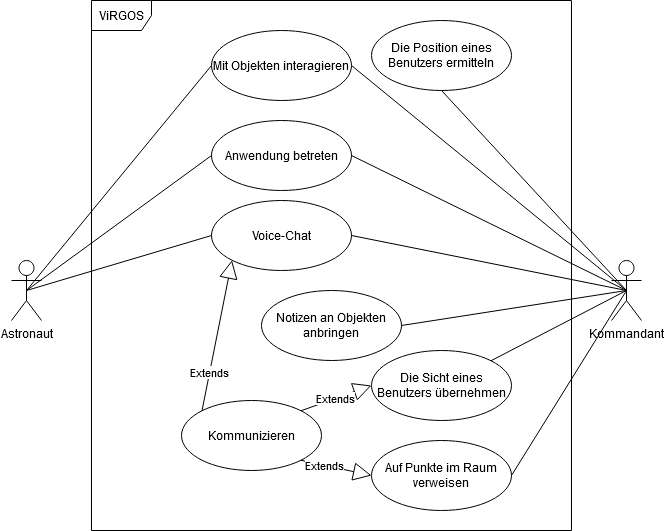
\includegraphics[width=1\textwidth]{ViRGOS_UseCase.png}
\caption{Use-Case-Diagramm von ViRGOS}
\end{figure}

\subsubsection{Nicht-Funktionale Anforderungen}
Die Nicht-Funktionalen Anforderungen geben Charakteristiken an, die in unterschiedlichem Maße in allen Projekten vorkommen.

\subsubsection*{Funktionalität}
Die Funktionen, um welche die Anwendung erweitert wird, sollen zum Erreichen des Ziels dieser Arbeit beitragen. Durch die experimentelle Natur dieser Thesis müssen die implementierten Funktionalitäten nicht final sein, sondern können in der Zukunft erweitert oder angepasst werden. Da zu jedem Zeitpunkt mehrere Studierende an unterschiedlichen Teilen dieses Projekts arbeiten, müssen spätestens bei der Zusammenführung Anpassungen vorgenommen werden.

\subsubsection*{Zuverlässigkeit}
Da das Ziel der Anwendung die Kooperation von mehreren Benutzern ist, muss jede Interaktion mit Objekten zuverlässig über alle Instanzen synchronisiert werden. Wenn ein Benutzer einen Knopf drückt um zum Beispiel eine Tür zu öffnen, und sich diese bei einem anderen Benutzer nicht auch öffnet, kommt es zu einer Diskrepanz in der Spielwelt. Dies kann zu einer Erschwerung in der Kommunikation führen, wenn Unsicherheit darüber besteht ob alle Benutzer exakt dasselbe sehen. Die Fehlertoleranz der Anwendung kann im Falle der Synchronisation von Positionen etwas höher sein, da diese Informationen mehrmals pro Sekunde abgeglichen werden. Bei einmaligen Benutzungen von Werkzeugen muss dies allerdings geringer ausfallen.
Da in der Anwendung keine Daten gespeichert werden gibt es keinen Grund einen Fokus auf Wiederherstellbarkeit im Fehlerfall zu setzen. Auch im Bezug auf Verfügbarkeit gibt es große Toleranzen da die Anwendung, aufgrund der notwendigen Einrichtung der Hardware, nur unregelmäßig verwendet wird.

\subsubsection*{Gebrauchstauglichkeit}
Da die Anwendung primär von Experten der Materie benutzt wird, und alle Laien von Experten begleitet werden, muss die Anwendung nicht zwingend einfach zu erlernen sein. Es sollte keine große Anfälligkeit für Fehler von Seiten der Benutzer geben, da sie nur eine begrenzte Menge an Funktionen zur Verfügung haben und die Experten des Labors einer falschen Benutzung vorbeugen. Da es sich bei dieser Arbeit um eine Virtual Reality Anwendung handelt, gibt keine Anforderungen an das Benuter-Interface, da die Anwendung optimalerweise gänzlich ohne ein Interface auskommt. 

\subsubsection*{Sicherheit}
Sicherheit ist bei diesem Projekt keine große Priorität, da die Anwendung exklusiv von Mitgliedern des Virtual Reality Labors benutzt wird. Somit haben Außenstehende keinen Zugriff auf die Soft- oder Hardware, weshalb zusätzliche Maßnahmen zur Stärkung der Sicherheit nicht notwendig sind.

\newpage

\subsubsection*{Effizienz}
Die Anwendung muss Änderungen sehr schnell über alle Instanzen synchronisieren um eine Immersion der Benutzer zu gewährleisten. Durch zu große zeitliche Abweichungen in der Datenübertragung kann es zu Asymmetrien in den Instanzen kommen, was die Zusammenarbeit erschweren kann. Des Weiteren muss die Anwendung genügend Kapazitäten für die Benutzer anbieten. Da das Ziel dieser Arbeit nur zwei Benutzer gleichzeitig vorsieht, halten sich die notwendigen Kapazitäten relativ niedrig. 

\subsubsection*{Wartbarkeit}
Da das Projekt auf der Arbeit von anderen Kommilitonen basiert und in Zukunft eventuell weiterentwickelt und erweitert werden soll, ist die Erweiterbarkeit eine wichtige Anforderung. Auch für abgewandelte Tests die in Zukunft durchgeführt werden könnten ist beispielsweise eine dynamische Anpassung an unterschiedliche Spielerzahlen unumgänglich.

\subsubsection*{Portabilität}
Da die Anwendung von spezieller Hardware, namentlich einem Virtual Reality Headset und einem Virtualizer, abhängt, gibt es keine große Anforderungen an die Portabilität. Die Software wird voraussichtlich nur im Rahmen des Virtual Reality Labors verwendet, und muss selten auf anderer Hardware installiert werden.

\subsubsection*{Kompatibilität}
ViRGOS interagiert ausschließlich mit anderen Instanzen von sich selbst. Somit muss die Anwendung mit keinem anderen Programm kompatibel sein. Es muss allerdings eine Koexistenz mit der Treibersoftware, die die notwendige Hardware kontrolliert, möglich sein. 

\newpage

\subsection{Auswahl der Technologien}
Aufgrund der Tatsache dass ViRGOS in Unity entwickelt wurde und als Basis für diese Arbeit dient, wird Unity auch hier als Entwicklungsumgebung verwendet. Um die Mehrspieler-Funktionalitäten umzusetzen, wurden die Möglichkeiten von UNet, Unitys eigener Mehrspieler-Lösung, geprüft. Unglücklicherweise ist UNet überholt und soll in naher Zukunft entfernt werden. Somit musste sich für eine Framework-Alternative entschieden werden.

\subsubsection{Mirror}
Eine mögliche Lösung stellte Mirror dar. Dieses Framework ist für große Spielerzahlen ausgelegt, die in ViRGOS nicht vorkommen werden. Zudem bietet Mirror eine große Menge an Werkzeugen für die Netzwerk-Entwicklung, ist aber dadurch nicht so anfängerfreundlich wie die Alternative. Die Architektur von Mirror sieht die Entwicklung eines Servers vor, der die Anwendung für die einzelnen Clients hostet. Da dies zusätzlichen Aufwand und Ressourcen benötigen würde, ist Mirror nicht optimal für dieses Projekt geeignet. 

\subsubsection{Photon}
Eine weitere Option ist Photon. In diesem Framework wird die Anwendung auf einem Cloud-Server gehostet, was den Zugriff von überall ermöglicht und die Verbindung zwischen Clients vereinfacht. Zudem ist das Framework weit verbreitet was eine große Wissensgrundlage und Hilfestellungen bietet. Des Weiteren bietet Photon eine kostenlose Version, die nur in der Größe der Cloud Server eingeschränkt ist, aber sonst alles bietet was für die Umsetzung dieses Projektes gebraucht wird. Somit wurde Photon für die Umsetzung gewählt. 

\newpage

\subsection{Entwurf}
Das Kapitel des Entwurfs beschreibt die Entwicklung der Konzepte von sowohl eines Prototypen als auch der eigentlichen Funktionalitäten in ViRGOS. Die Entwürfe bezüglich ViRGOS sind in die Mehrspielerfähigkeit der Anwendung im Allgemeinen und die Werkzeuge für die Kooperation gegliedert. Abschließend wird ein Entwurf für Tests der Anwendung und eine Befragung von Probanden im Rahmen einer Studie vorgestellt.

\subsubsection{Prototyp}
Um sich mit Unity und Photon vertraut zu machen soll anfangs ein Prototyp entwickelt werden. Hier soll getestet werden wie mit Photon eine Lobby für mehrere Spielern erstellt werden kann. Anschließend sollen einfache Interaktionen mit Objekten implementiert werden. Wenn mehrere Benutzer die Anwendung gleichzeitig verwenden und mit Objekten interagieren können, soll getestet werden wie mit Kollisionen umgegangen werden kann. Hierbei sind Kollisionen mehrerer Interaktionen gemeint, also mehrere Benutzer die gleichzeitig versuchen auf ein Objekt zuzugreifen. Zudem soll die Synchronisation von Zuständen getestet werden. Wenn ein Benutzer mit einem Objekt interagiert und dieses Objekt beispielsweise seine Position ändert, muss dies auch bei allen anderen Benutzern passieren. 


\subsubsection{Mehrspielerfähigkeit in ViRGOS}
Zu Beginn soll ViRGOS um Photon erweitert werden, um mehreren Benutzern den gleichzeitigen Zugriff auf die Anwendung zu ermöglichen. Die Avatare sollen instanziiert werden sobald ein Benutzer beitritt. Somit ist die Anzahl der Benutzer dynamisch und muss nicht im Voraus festgelegt werden. Die Anwendung ist zwar für zwei Benutzer ausgelegt, kann aber in Zukunft weiterentwickelt werden. Somit sollte die Option von mehr als zwei Benutzern offen gehalten werden. Um eine Anweisung des Astronauten durch den Kommandanten notwendig zu machen soll eine Aufgabe für den Astronauten implementiert werden. Diese Aufgabe soll komplex genug sein, dass eine Anweisung über den Voice-Chat nicht immer ausreicht. Um die Verwendung von weiteren Werkzeugen notwendig zu machen, soll sich der Aufbau, der die Aufgabe darstellt, außerhalb der Rakete befinden. 

\subsubsection{Werkzeuge}
Um die aktuelle Position des Astronauten zu ermitteln, soll der Kommandant die Möglichkeit haben sich das Sichtfeld des Astronauten auf einem der Bildschirme anzeigen zu lassen. Somit weiß der Kommandant vor welchem Problem sich der Astronaut gerade befindet. Da die Bildschirme der Kommandozentrale relativ hoch platziert und nicht sehr groß sind, reichen diese nicht aus um kleine Details wahrzunehmen. Ein weiteres Werkzeug das dem Kommandanten zur Verfügung stehen soll, ist die Möglichkeit sein eigenes Sichtfeld durch das des Astronauten zu ersetzen. Somit wird nicht nur auf einem kleinen Bildschirm dargestellt was der Astronaut sieht, sondern es wird möglich durch die Augen des Astronauten zu sehen. Somit verfügt der Kommandant über dieselben Informationen wie der Astronaut, ohne dass dieser alles über den Voice-Chat schildern muss. \\

\noindent Um Informationen an den Astronauten zu übermitteln sollen dem Kommandanten neben dem Voice-Chat verschiedene Werkzeuge zur Verfügung stehen. Es soll ein Zeiger-Werkzeug implementiert werden, dass es ermöglicht auch aus einiger Entfernung auf einen bestimmten Punkt zu verweisen. Somit können präzise Anweisungen an den Astronauten übermittelt werden. Um dies auch dann zu ermöglichen wenn sich beide Nutzer nicht in nächster Nähe befinden, soll sich das Zeiger-Werkzeug auch verwenden lassen, wenn der Kommandant den Bildschirm verwendet und das Sichtfeld des Astronauten verwendet. Dies ermöglicht dem Kommandanten auf einen bestimmten Punkt im Sichtfeld des Astronauten hinzuweisen. \newline

Ein weiteres Werkzeug zur Übermittlung von Informationen an den Astronauten ist die Möglichkeit Notizen zu erstellen und zu platzieren. Der Kommandant soll eine neue Notiz anlegen und diese über eine Virtual Reality Tastatur mit Text befüllen können. Diese fertige Notiz soll dann für den Astronauten sichtbar an Objekten platziert werden können. Somit können wichtige Informationen mit Bezug auf ein Objekt in der Szene auf Abruf an den Astronauten übermittelt werden. Dies kann besonders für schwer zu merkende Informationen nützlich sein die mehrmals gebraucht werden. 

\subsubsection{Tests und Befragungen}
Bereits während der Entwicklung an ViRGOS sollen Tests mit Probanden durchgeführt werden. Diese Personen sollen unterschiedliche Mengen an Erfahrungen mit Virtual Reality Anwendungen haben. Die Tests sollen Aufschluss darüber geben, ob die implementierten Funktionen intuitiv zu benutzen sind oder weiterer Anpassung bedürfen. 

Nach Abschluss der Entwicklung soll eine Befragung mit mehreren Teilnehmern durchgeführt werden. Die Teilnehmer sollen mit einem Virtual Reality Headset, in der Rolle des Astronauten, die Anwendung betreten. Unter Anleitung des Kommandanten sollen sie die Rakete über den Aufzug verlassen und sich zu dem Testaufbau begeben. Dort angekommen sollen sie die Aufgabe durchführen. Um die Unterschiede der Werkzeuge zu testen, sollen die Tests unterschiedlich ablaufen.

\begin{itemize}
\item[Test 1]  Der Astronaut soll nur über den Voice-Chat und ohne den Bildschirm angeleitet werden
\item[Test 2]  Der Astronaut soll nur über den Voice-Chat mit dem Bildschirm angeleitet werden
\item[Test 3]  Der Astronaut soll nur mit dem Zeiger-Werkzeug und dem Notizen-Werkzeug über den Bildschirm angeleitet werden
\item[Test 4]  Der Astronaut soll über den Voice-Chat UND mit den Werkzeugen angewiesen werden
\end{itemize}

Anschließend sollen die Probanden Fragen beantworten, die Auskunft über die Effektivität der unterschiedlichen Unterweisungen geben. Jeder Proband soll alle Tests durchlaufen. Somit kann jeder Proband die Unterschiede zwischen den Methoden und eventuell die eigenen Präferenzen schildern. Die Reihenfolge der Tests soll bei jedem Probanden rotieren. Somit kann eine Befangenheit des Probanden verhindert werden, was zu ungenauen Ergebnissen bei den späteren Tests führen kann. \newline

Diese Chance soll zudem genutzt werden, um das Basissystem ViRGOS zu evaluieren. Die Benutzer sollen die Benutzbarkeit der Anwendung und den Grad der Immersion im allgemeinen bewerten. Außerdem sollen sowohl das Kransystem als auch der Virtualizer von den Benutzern bewertet werden. 

Eine weitere Erkenntnis die aus diesen Tests gewonnen werden kann sind potentielle Unterschiede in der Immersion des Kommandanten. Die Hälfte der Tests soll durchgeführt werden während der Kommandant ein Virtual Reality Headset trägt. Bei der anderen Hälfte befindet sich der Kommandant an einem Computer und steuert seinen Avatar über die Maus und Tastatur. Ihm stehen in beiden Fällen sämtliche Werkzeuge zur Verfügung. Hiermit soll ermittelt werden ob eine Immersion des Kommandanten während der Anleitung des Astronauten vorteilhaft ist. Der hierzu entwickelte Fragebogen befindet sich im Anhang dieser Arbeit.
